\documentclass[onecolumn, draftclsnofoot,10pt, compsoc]{IEEEtran}
\usepackage{graphicx}
\usepackage{setspace}
\usepackage{comment}
\usepackage{bigstrut}
\usepackage{geometry}
\usepackage{supertabular}
\usepackage{tabu}
\usepackage{hyperref}
\usepackage{url}
\hypersetup{
  colorlinks=true, linkcolor=blue, citecolor=blue, filecolor=blue, urlcolor=blue}
\geometry{textheight=9.5in, textwidth=7in}

% 1. Fill in these details
\def \CapstoneTeamName{		Remix}
\def \CapstoneTeamNumber{		61}
\def \GroupMemberOne{			Josh Matteson}
\def \GroupMemberTwo{			Steven Powers}
\def \GroupMemberThree{			Evan Tschuy}
\def \CapstoneProjectName{		Many Voices Platform}
\def \CapstoneSponsorCompany{	Oregon State University}
\def \CapstoneSponsorPerson{		Carlos Jensen}

% 2. Uncomment the appropriate line below so that the document type works
\def \DocType{
				%Abstract
		        %Problem Statement
				%Requirements Document
				%Technology Review
				Design Document
				%Progress Report
				}

\newcommand{\NameSigPair}[1]{\par
\makebox[2.75in][r]{#1} \hfil 	\makebox[3.25in]{\makebox[2.25in]{\hrulefill} \hfill		\makebox[.75in]{\hrulefill}}
\par\vspace{-12pt} \textit{\tiny\noindent
\makebox[2.75in]{} \hfil		\makebox[3.25in]{\makebox[2.25in][r]{Signature} \hfill	\makebox[.75in][r]{Date}}}}
% 3. If the document is not to be signed, uncomment the RENEWcommand below
\renewcommand{\NameSigPair}[1]{#1}

%%%%%%%%%%%%%%%%%%%%%%%%%%%%%%%%%%%%%%%
\begin{document}
\begin{titlepage}
    \pagenumbering{gobble}
    \begin{singlespace}
    	
\includegraphics[height=4cm]{coe_v_spot1}
        \hfill
        % 4. If you have a logo, use this includegraphics command to put it on the coversheet.
        %\includegraphics[height=4cm]{CompanyLogo}
        \par\vspace{.2in}
        \centering
        \scshape{
            \huge CS Capstone \DocType \par
            {\large\today}\par
            \vspace{.5in}
            \textbf{\Huge\CapstoneProjectName}\par
            \vfill
            {\large Prepared for}\par
            \Huge \CapstoneSponsorCompany\par
            \vspace{5pt}
            {\Large\NameSigPair{\CapstoneSponsorPerson}\par}
            {\large Prepared by }\par
            Group\CapstoneTeamNumber\par
            % 5. comment out the line below this one if you do not wish to name your team
            \CapstoneTeamName\par
            \vspace{5pt}
            {\Large
                \NameSigPair{\GroupMemberOne}\par
                \NameSigPair{\GroupMemberTwo}\par
                \NameSigPair{\GroupMemberThree}\par
            }
            \vspace{20pt}
        }
        \begin{abstract}
        % 6. Fill in your abstract
		\noindent The Many Voices Publishing Platform uses a variety of
		 technologies to handle different aspects of the project, from 
		 the user interface to the back-end database operations. 
		 This document covers these technologies and follows the process
		 that enable to the Many Voices Publishing Platform to succeed 
		 in delivering a working platform for textbook collaboration.
        \end{abstract}
    \end{singlespace}
\end{titlepage}
\newpage
\pagenumbering{arabic}
\tableofcontents
% 7. uncomment this (if applicable). Consider adding a page break.
%\listoffigures
%\listoftables
\clearpage


% 8. now you write!
\section{Revision Log}
\begin{flushleft}
\tablehead{}
\begin{supertabular}{|p{3cm}|p{3cm}|p{3cm}|p{7cm}|}
\hline
Name & Change Number & Date & Description of Change  
\\\hline
Steven Powers & 1 & 2/14/2017 & Updated document to use new style.
								Improved readability of Latex and PDF
								documents. Removed definitions for Federated
								and Wiki, as they were not used in the 
								document.
\\ \hline

\end{supertabular}
\end{flushleft}

\section{Overview}
\noindent The Software Design Document is a document to provide aid
for the software development process by providing detailed information
on how the software should be built. Additionally providing information
on interactions between different pieces of software and users through
use cases, UML diagrams, and other supporting information.

\subsection{Scope}
\noindent This Software Design Document is used to record design
information and communicate design information to project stakeholders.
This Software Design Document also provides the details of required
functionality for the Many Voices Publishing Platform, a textbook creation
platform for publishing textbooks.

\subsection{Purpose}
\noindent The purpose of this document is to describe the implementation
of the Many Voices Publishing Platform (MVP Platform) software.
The Many Voices Publishing platform is designed to allow for the creation
of textbooks by College and University professors or any person interested
in creating their own textbook.

\subsection{Intended Audience}
\noindent This document is intended for Professor D. Kevin McGrath,
Dr. Kirsten M. Winters, and PhD Student Jonathan Dodge of Oregon State
University for curriculum grading purposes.
Additionally this document is intended for Dr. Carlos Jensen for the
purpose of client information and senior capstone project purposes.

%Section 2
\section{Definitions}
\begin{center}


\begin{supertabular}{p{3cm}p{12cm}}

	Aurelia 
	& A JavaScript client framework for mobile, desktop and web leveraging
	simple conventions and empowering creativity \cite{Aurelia}. \\

	Alpha Test 
	& Limited release(s) to selected, outside testers (Friends and Family)\\

	Beta Test 
	& Limited release(s) to cooperating customers wanting early
	access to developing systems (Professors and other educators)\\

	Final Test 
	& Release of full functionality to customer for approval \\

	PDF 
	& Portable Document Format, that is able to combine text,
	graphics, and other information into a single document \\

	PCI 
	& Payment Card Industry, is a proprietary information security
	standard for credit cards in an effort to reduce credit card fraud \\

	Scrap 
	& A section of a textbook, which can contain formatted text 
	(markdown or latex), and media \\

	Section 
	& An ordered collection of Scraps belonging to a chapter\\

	Chapter 
	& An ordered collection of Sections and Scraps\\

	SDD 
	& Software Design Document \\

	SSRS 
	& System and Software Requirements Specification \\

	Source Control 
	& An element of software design management, version control, and 
		is the management of changes to documents, large web sites, 
		computer programs, and other collections of data \\

	Media 
	& A standalone image, figure, or video. Can be embedded in a Scrap\\

	Node 
	& A JavaScript runtime designed to build scalable network applications\\

	UML 
	& Unified Modeling Language -- A general purpose, development 
	modeling language in the field of computer science\\

	UI  
	& User Interface -- The means by which the user and a 
	computer system interact, in particular the use of input 
	devices and software\\

	Web Application 
	& An interactive program that can be accessed and is based through 
	a web server instead of being stored on a user's desktop\\

\end{supertabular}

\end{center}



%Section 3
\section{Conceptual model for software design descriptions}
%{\noindent  \par}


%\subsection{Software design in context}
%{\noindent  \par}

\subsection{Software design descriptions within the life cycle}
\noindent The Software Design Description (SDD) is based in large part upon
the System and Software Requirements Specification (SSRS) document.
Requirements listed within the SSRS influence details within the SDD and
the SDD may influence the SSRS details. \\


%Section 4
\section{Design Description}


\subsection{Introduction}
\noindent When designing software to handle the creation of a textbook,
the technologies in the background are equally as necessary as those in 
the foreground. The creation of a textbook requires various systems 
and technologies to handle the storing and presentation of data to allow 
the user to create their project.\\

%\subsection{SDD identification}
%{\noindent \par}

\subsection{Design Stakeholders}
\noindent The stakeholders consist of Dr. Carlos Jensen, members of the Oregon
State University senior capstone educational team, including Professor 
D. Kevin McGrath, Dr. Kirsten M. Winters, and PhD student Jonathan Dodge.
Additional stakeholders include the development team consisting of 
Steven Powers, Evan Tschuy, and Josh Matteson.\\

\subsection{Design Concerns}
\noindent The design concerns for this project include the building of a 
User Interface with a functional JavaScript framework that allows for 
ease of use for users and developers. \\

\noindent User login and authentication will also be a design concern for 
this project, as preventing unintended access to another users work is 
very important. \\

\noindent Another concern consists of the usability of the interface 
and being able to inform the user of actions they expect to perform and can perform to complete their task of creating a textbook. \\

\subsection{Design Views}
\noindent The SDD will use UML diagrams to describe and visualize aspects of the design. \\

\subsection{Design Viewpoints}
\noindent This SDD will cover a number of different viewpoints, including:
context, composition, logical, dependency, information, interface, 
and interaction viewpoints. \\

\medskip 

\noindent Context viewpoints cover the relationships, dependencies, and
interactions between the system and its environment \cite{viewpoints}. \\

\medskip 

\noindent Composition viewpoints cover what information will be handled 
by the software. \\

\medskip 

\noindent Logical viewpoints cover what purpose the software will serve 
and how the software will achieve this purpose. \\

\medskip 

\noindent Dependency viewpoints cover outside elements that need to 
be integrated into the software in some way, as the implementation will 
depend on these outside elements. \\

\medskip 

\noindent Information viewpoints cover data that is present within 
the software or managed by the software in some way. \\

\medskip 

\noindent Interface viewpoints cover how designers and developers will 
be using the software, detailing the internal and external interfaces of 
the software. \\

\medskip 

\noindent Interaction viewpoints cover the interactions between different entities or elements within the software. \\

\subsection{Design Elements}
\noindent Design elements within our software will include a variety 
of different features that are often considered standard elements 
within software. These elements include buttons, text boxes, search boxes, 
menus, and clickable links just to name a few. The menus of the system will be 
limited for user convenience and will provide a meaningful icon or text 
representation for quick affordability for the user. Within the text editing 
area, the user will be able to arrange text how they would like it to appear 
in a finalized---compiled version. \\

\noindent The text area will also allow users to specify other documents to 
include, which will be handled by the software in the background at time of 
compilation. Each included document or file will be stored as a separate 
document with version control capabilities. \\

%\subsection{Design Overlays}
%{\noindent \par}

\subsection{Design Rationale}
\noindent For this project, design choices are made based on client 
specifications as well as development concerns due to technology availability 
and adaptability to the current system. Our client Dr. Carlos Jensen wants the 
project to allow for the easy creation of textbooks through what is called the 
Many Voices Publishing Platform. Design choices will be made to accommodate 
this requirement.


\newpage
\subsection{Design Timeline}
\begin{figure}[ht!]
\centering
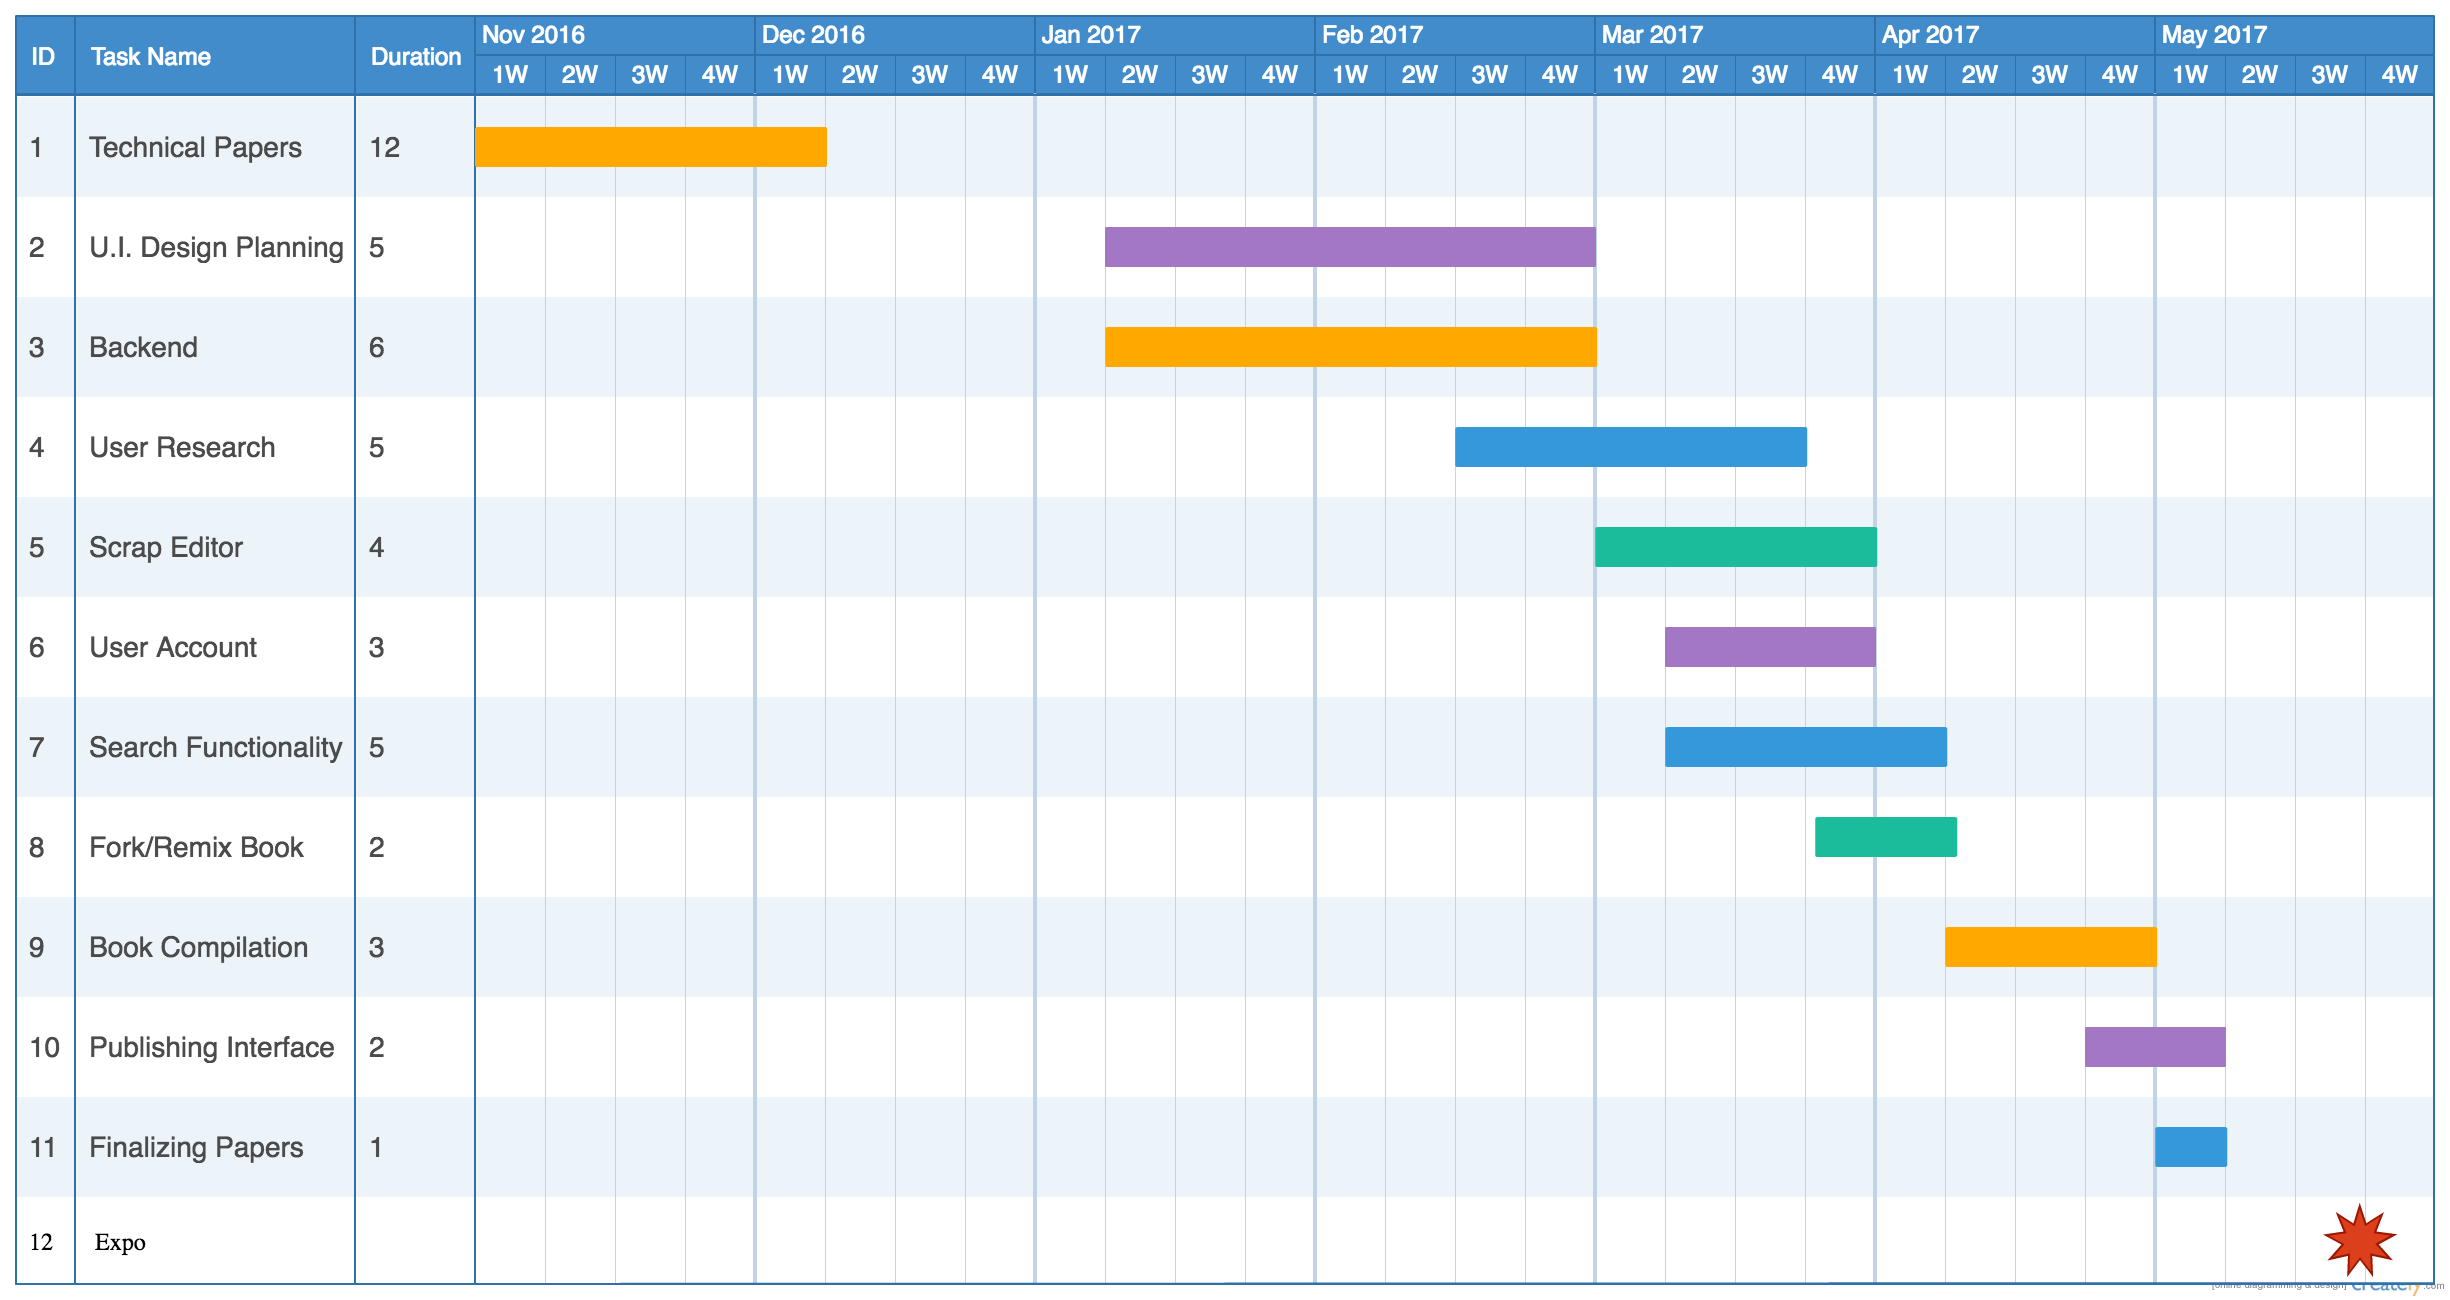
\includegraphics[width=160mm]{gantt_chart.png}
\caption{A preliminary Gantt Chart that outlines a rough sketch of our anticipated working time line as of Fall term}
\end{figure}

\subsection{Design Languages}
{\noindent This document will use UML as the design language.\par}





\clearpage
%Section 6
\section{Design Viewpoints}

\subsection{Introduction}
\noindent This section will cover: context, composition, logical, dependency, information, interface, and interaction viewpoints. 

\noindent Steven Powers is covering User Interface Tools, 
User Login \& Authentication, and Interface Design.  \\
\noindent Evan Tschuy is covering Server Back-end, Text Formatting, 
and Password Storage. \\
\noindent Josh Matteson is covering Testing, Revision Control Software, 
and Database. \\


%Steven's Section

\subsection{Viewpoint: User Interface Tools}
{\noindent By: Steven Powers \par}

\subsubsection{Interface}
\noindent The user interface is one of the most important parts to the Many
Voices Publishing Platform. An easy to use UI can make the difference between
two competing software solutions. The Many Voices Publishing Platform will be
interacted through a website that will display a users documents and their 
current document. The User Interface Tools will allow for a high quality user 
experience with a high number of screen repaints per second, further 
increasing the ease of use with the software through a fluid user interface 
\cite{Eisenberg}. \\

\subsubsection{Design Concerns}
\noindent A poorly implemented UI can result in users choosing a competing
product or simply deciding not to use any software for their intended purpose.
Users are often impatient and quick to abandon software, further proving the 
need for a robust and easy to use User Interface Toolset.  \\

\subsubsection{Design Elements}
\noindent The User Interface Tools will allow for scalability when it comes to
using the software on different platforms, including mobile, and desktop 
environments. Additionally the tools will provide great interact-ability for 
the user. \\

\subsubsection{Function Attribute}
\noindent This component provides the user interface for users to interact with while using the software. Handles display of information and provides the interface for input. \\

\subsubsection{Relationship}
\begin{figure}[ht!]
\centering
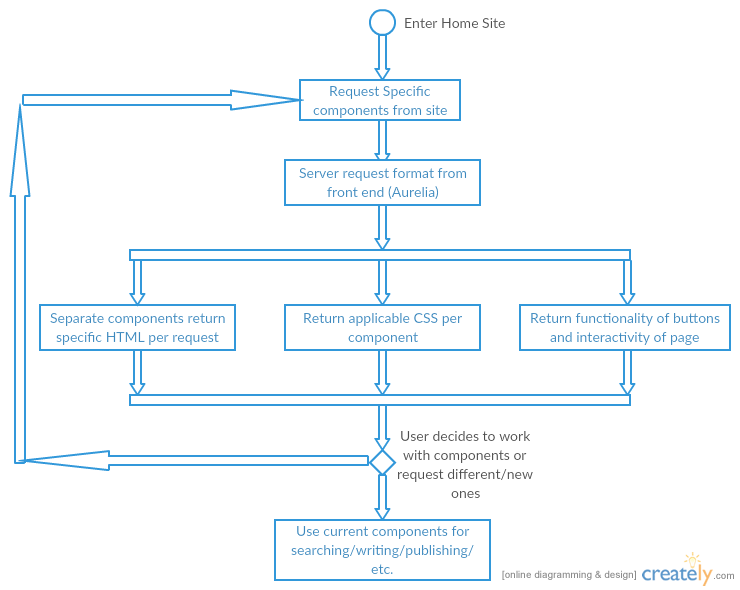
\includegraphics[width=140mm]{user_interface_tools.png}
\caption{A preliminary UML diagram of how the user interface tool of
	Aurelia will enable transmission of data to the screen or from the 
	screen, up to date as of Fall term}
\end{figure}

\newpage
\subsection{Viewpoint: User Login \& Authentication}
\noindent By: Steven Powers \\

\subsubsection{Context--Dependency}
\noindent A user login system is standard affair for most websites on the 
Internet. How these user logins take place and authenticate users can vary 
quite significantly depending on the implementation. User login security is 
important for protecting the customer as well as the reputation of the 
software and company. User Login \& Authentication are dependent on Evan 
Tschuy's section on Password Storage section. \\

\subsubsection{Design Concerns}
\noindent Handling user logins and user authentication can be quite a painstaking process, as any mistake can cost you customers and any reputation that was present before the mistake was exploited. Authentication, or the matching of user submitted data with our stored credentials can be exploited though a simple MySQL command, if our servers are not secured properly. In house solutions can be buggy, or not as secure. Third party solutions require an account with those services and has security in their hands.

\subsubsection{Design Elements}
\noindent A way to login securely, through created credentials or through a
third party login system, such as Login with Facebook or Google. \\

\subsubsection{Function Attribute}
\noindent This component provides the functionality of user login process
and user authentication within the software. \\



\subsection{Viewpoint: Interface Design}
\noindent By: Steven Powers \\

\subsubsection{Information}
\noindent The approach for user interface design is quite different
than that of the tools being used. Interface Design refers to the
methodologies employed to create the UI. This often takes the form of
user studies, and demoing of prototypes and release candidate mockups
for feedback. For our software, our target audience is professors,
especially those interested in publishing their own book currently or
in the near future. Using the target audience as a design requirement,
the designer is able to gleam a lot of information about how to best
serve this user. Methodologies include user centered design, activity 
centered design, and self design principles to list a few common 
disciplines. \\

\subsubsection{Design Concerns}
\noindent Interface Design is an often overlooked portion of any software 
product. For some software products it would be no surprise that the software 
is never used in house, we are trying to avoid this feeling.
User centered design, while often the standard for the Computer Science 
industry, it very costly, both in terms of time and money. There is a large 
amount of time into user research studies and live demos. Self design, while 
much faster, and easier to perform, can lead to results that do not satisfy 
your users expectations.\\

\subsubsection{Design Elements}
\noindent An Interface Design methodology that allows for efficient
use of time as well as successful design choices to best suit our users. \\

\subsubsection{Function Attribute}
\noindent Provides methodologies for improving Interface Design to assist
users and developers. \\

\newpage
\subsubsection{Relationship}
\begin{figure}[ht!]
\centering
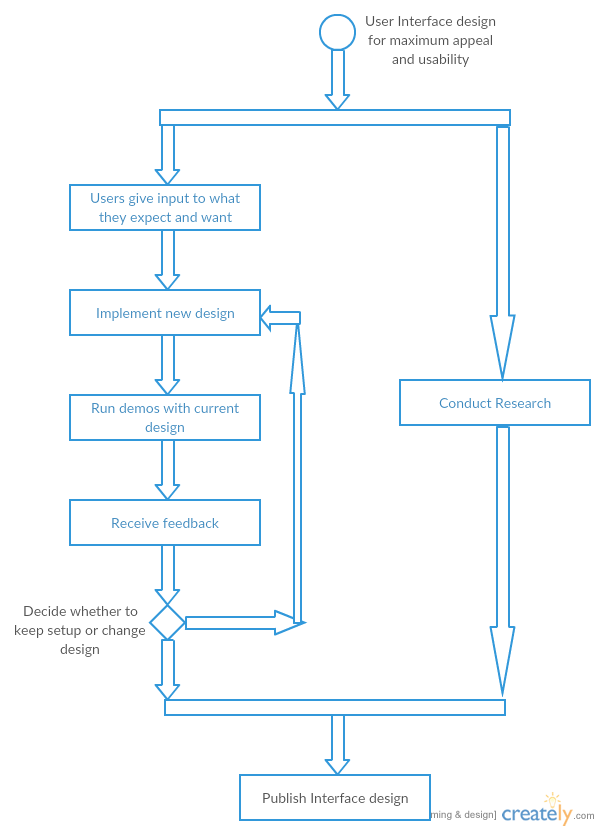
\includegraphics[width=120mm]{interface_design.png}
\caption{A preliminary UML diagram of how user centered design \& user research can
improve a UI for increased affordance and usability for the target
audience, up to date as of Fall term}
\end{figure}





%Evan's Section
\newpage
\subsection{Viewpoint: Server Back-end}
\noindent By: Evan Tschuy \\

\subsubsection{Backend}
\noindent
A standard web application follows more or less a standard design flow. 
When a request is received, a URL parser parses the URL and passes it to the 
appropriate function, along with all of its parameters. The function then 
operates on the data somehow, and returns either the result of a template 
render or a block of data in JSON/XML to be returned to the client. Inside the 
function, the heavy lifting of data manipulation, 
storage, etc. takes place. \\


\subsubsection{Design Concerns}
\noindent The main concern for the backend of the project is how the back end 
will communicate with the version control system. For instance, building on 
top of Git, it is necessary to also verify that the backend language chosen 
has a library that can be used to easily interact with Git. Then, it will be 
necessary to build an internal library that can be placed on top of Git that 
exposes only the operations needed for the textbook project. \\

\subsubsection{Design Elements}
\noindent The backend design, especially the layer interacting with Git, will 
play a critical role in speed of development. By implementing a Snippet and 
Textbook super-layer on top of the existing Git library, we can eliminate 
having to think about Git as early as possible, and spend our time instead on 
interacting with Snippets and the Textbooks.\\

\subsubsection{Function Attribute}
\noindent This function provides the base on which the rest of the project is
built — the interaction layer between the frontend and the revision control 
system.


\newpage
\subsubsection{Relationship}
\begin{figure}[ht!]
\centering
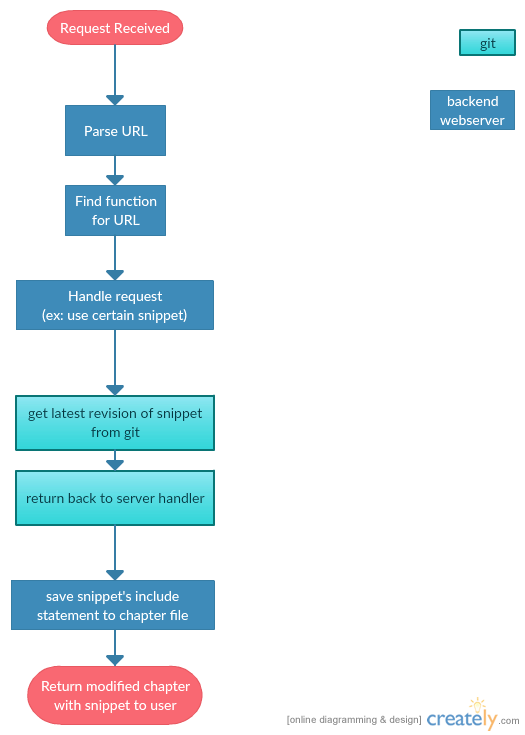
\includegraphics[scale=0.5]{backend.png}
\caption{An example backend handling flow. The application determines which 
function to call, and the function handles the request and sends any necessary 
file operations to the git module.}
\end{figure}
\pagebreak





\subsection{Viewpoint: Text Formatting}
{\noindent By: Evan Tschuy \par}

\subsubsection{Formatting}
\noindent The front end of the platform lets users interact with "snippets" of 
documents — a block of text that, paired with potentially dozens of other 
snippets, can make a chapter. Then, chapters need to be combined together to 
make a full textbook. Using a LaTeX back-end, snippets can be related to an 
\begin{verbatim}\input{}\end{verbatim} command, which takes the raw commands 
of a document and puts them into another document. Chapters can be related to 
\begin{verbatim}\include{}\end{verbatim} commands, which start a new page and 
add the new section. In this way, we can have one file for the table of 
contents, which controls which chapters are included in which order, and one 
file for each chapter, which controls which snippets are included in which 
order. \\

\iffalse
\noindent Users expect to be able to add things to documents like bolded text, 
tables, etc. From a design perspective, this means adding an intermediary step 
between what a user can use as input, and how that gets stored as plain text 
in a raw document on the backend. Already today many web-based LaTeX and 
Markdown editors exist, and so the goal for the platform will be to integrate 
an existing editor into the user interface in a friendly way. \fi

\subsubsection{Design Concerns}
\noindent The files referenced are all stored in version control, as discussed 
below. Therefore we need to relate the files to a specific version as stored. 
Additionally, it needs to be entirely invisible to users how the text is being 
split — the users should not know whether the backend is written in LaTeX 
using include and input statements, or in Markdown with string concatenation, 
or any other possible implementation. \\
\iffalse
A user cannot know how their text is being transformed between what they can
interact with on the front end and how it is being stored in the back end. 
This means the user should only ever have to deal with a "rich text" editor, 
like those found in Microsoft Word or Google Docs, with the ability to do all 
text manipulation with convenient nearby buttons.
\fi

\subsubsection{Design Elements}
\noindent An abstraction of snippets and chapters into LaTeX documents in 
such a way as to make manipulation of them individually and as a whole simple.
\\

\subsubsection{Function Attribute}
\noindent This component provides the functionality of document generation, 
storage, and manipulation. \\

\subsubsection{Relationship}
\begin{figure}[ht!]
\centering
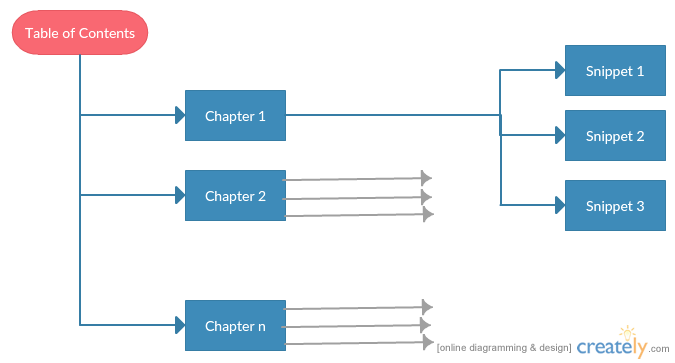
\includegraphics[scale=0.5]{formatting.png}
\caption{A document is divided into chapters (which are included under a 
table of contents) and snippets (which are parts of a chapter).}
\end{figure}
\pagebreak

\subsection{Viewpoint: Password Storage}
\noindent By: Evan Tschuy \\

\subsubsection{Password hashing}
\noindent  Any time a password is being requested from a user, it should be 
securely and irreversibly hashed. By securely hashing a password, it becomes 
impossible for hackers with access to the user database to use stored 
credentials to compromise user accounts on other sites even if users reuse 
passwords between sites. A well designed cryptographic hash, such as bcrypt, 
includes a salt value, which is simply added to the beginning of the password 
at hash time, stored in the database in plain text, so that two uses of the 
same password result in different hashes. \\


\subsubsection{Design Concerns}
\noindent A secure password storage system always hashes passwords, and requires hackers to crack each password individually by guessing passwords one by one. Another alternative to storing user passwords at all is, as discussed above in the user authentication section, to use a third-party user authentication service such as those offered by Google, Facebook, etc. For a platform used by professors, who may not all have a Google or Facebook account, however, it should always be possible to create an account that does not require a third-party account. \\

\subsubsection{Design Elements}
\noindent A well-designed, secure system in which any password stored cannot 
be reversed without a slow cracking process. Preferably, users would not store 
any passwords at all with the service and instead would use third-party 
authentication. \\


\subsubsection{Function Attribute}
\noindent This component provides the functionality of secure password storage. \\


\subsubsection{Relationship}
\begin{figure}[ht!]
\centering
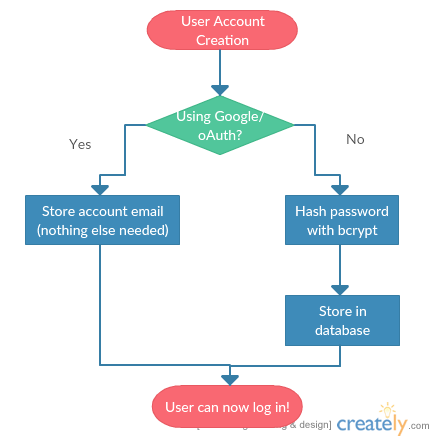
\includegraphics[scale=0.5]{password.png}
\caption{Passwords will either be securely hashed, if the user is not using external authentication, or not needed at all, if the user is using external authentication.}
\end{figure}
\pagebreak





%Josh's Section
\newpage
\subsection{Viewpoint: Testing}
{\noindent By: Josh Matteson \par}

\subsubsection{Information}
\noindent Testing is one of the most substantial parts when considering the 
success and thoroughness of an application. If not properly tested, the 
application will contain numerous bugs resulting in: faulty functionality, 
unpredictable behavior, and the pages not loading. \\


\subsubsection{Design Concerns}
\noindent The main concerns with working with a testing framework is the level 
of complexity and with that the learning curve.
Jasmine, existing for almost a decade, has had numerous contributors to its 
documenation. This ensures that, while making progress,
we won't be short of useful information in the furthest reaches of the 
internet. \\

\subsubsection{Design Elements}
\noindent Jasmine is open source, and therefore, will be used as the main testing framework for application.
It will be one of the developer dependencies and will mostly interact with the existing javascript/typescript of our application.
Jasmine will be ran through our node express backend, and will come with a coverage report for our app. Whether this is from Jasmine or
from another testing framework that works closely with it. \\

\subsubsection{Function Attribute}
\noindent Assist in development and thoroughness of the application. Will drastically reduce bugs. \\

\newpage
\subsubsection{Relationship}
\begin{figure}[ht!]
\centering
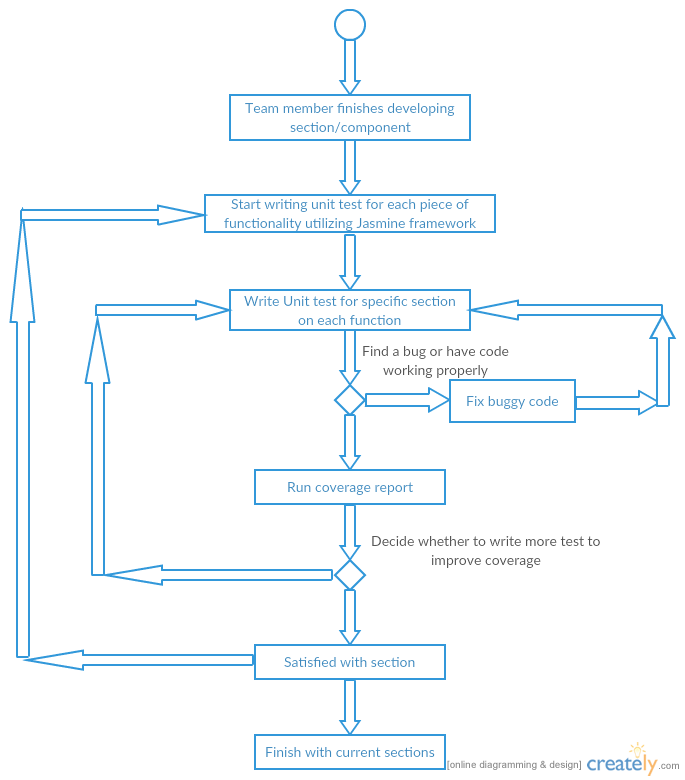
\includegraphics[width=120mm]{Testing.png}
\caption{A preliminary UML diagram demonstrating the flow of testing with Jasmine}
\end{figure}

\newpage
\subsection{Viewpoint: Revision Control Software}
{\noindent By: Josh Matteson \par}

\subsubsection{Revision Control}
\noindent One of the more important elements of our application, the revision 
control will let the user have full control over their current work and back 
ups. If the user realizes that a section they wrote conflicts with something 
someone else wrote,they can then backup from a previous version. This will all 
be done with Git as the background technology, which in essence, is the 
backbone of major web platforms like Github. This component will give users 
endless control with branches, previous versions, and much more. \\

\subsubsection{Design Concerns}
\noindent One of the main design concerns is properly integrating 
Git with the rest of the application. Ensuring that the flow from user to 
Git then to database will require well force all parts of the app to 
be working. \\


\subsubsection{Design Elements}
\noindent Git will act as middleware in between the front end and the back-
end, this will be taken into mind when moving forward. The user will use one 
of the front end functions, which will request an action of Git, and finally 
perform database operations. \\

\subsubsection{Function Attribute}
\noindent The overarching purpose of Git is to give users free reign to write 
whatever they want with little to no consequences from themselves or other users. \\

\newpage
\subsubsection{Relationship}
\begin{figure}[ht!]
\centering
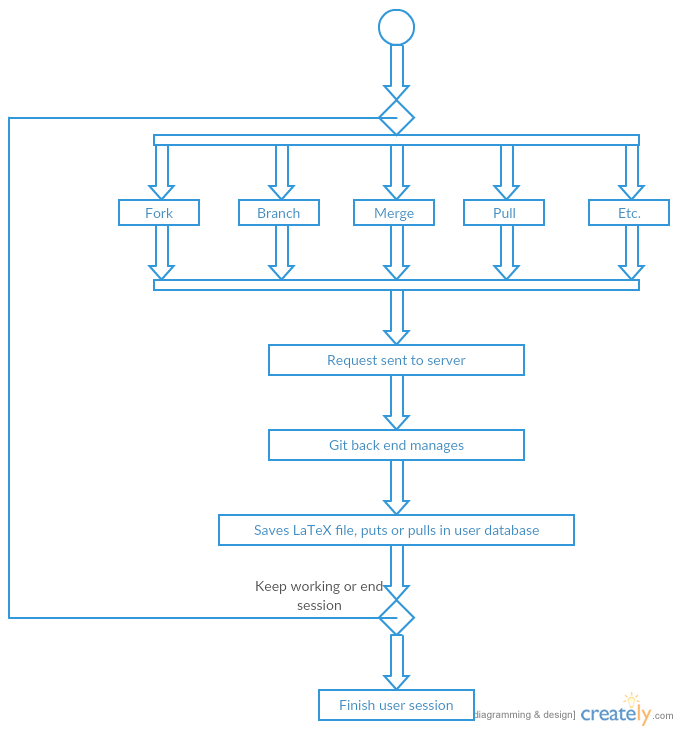
\includegraphics[width=120mm]{Revision_Control.png}
\caption{A preliminary UML diagram demonstrating the relationship of Git to the request of the user}
\end{figure}

\newpage

\subsection{Viewpoint: Database}
{\noindent By: Josh Matteson \par}

\subsubsection{Database}
\noindent While understanding what a database does is more common even 
among non computer science majors, the aspects of its relation
to other components of our application are not self explanatory. 
The database's most important role consist of storing user information,
and ensuring that information does get misplaced or skewed a long the way 
to the user. \\

\subsubsection{Design Concerns}
\noindent As with most databases, one of the main design concerns is 
the complexity of the calls to it. Some databases use a query structure,
other ones use explicit calls. SQL Server, as is part of the name, 
will be using query calls to receive information. \\

\subsubsection{Design Elements}
\noindent Our backend components, being Node.js and Express, will be doing 
the calls to the database. Front end functions will call general purpose
functions in the backend, which will then make a call to the database. This 
will then go back up the ladder to the user. \\

\subsubsection{Function Attribute}
\noindent The database stores all important information about the user 
and their revisions, passwords, and preferences. \\


%Section 10
\section{Conclusion}
{\noindent  The Many Voices Publishing Platform is a combination of User Interfaces, Documentation, User Centered Design, Testing, User Authentication, Databases, Server Back-end, Text Formatting, Password Storage, and the users themselves. Determining the technologies behind these parts and pieces is a difficult task to accomplish, as many choices can satisfy the requirements of the project. Finding the best solution however is the goal of this document, to provide a clear path forward for the platform as a whole. \par}



\newpage

%Section 7
%\section{Annex A - (information Bibliography)}

\nocite{*}
\bibliographystyle{IEEEtran}
\bibliography{designdocument}


%Section 8
%\section{Annex B - Conforming design language description}
%{\noindent \par}

%Section 9
%\section{Annex C - Templates for an SDD}
%{\noindent \par}







\end{document}
